
%(BEGIN_QUESTION)
% Copyright 2008, Tony R. Kuphaldt, released under the Creative Commons Attribution License (v 1.0)
% This means you may do almost anything with this work of mine, so long as you give me proper credit

Nedenfor ser du en membranstyrt {\it trykkbryter}, konstruert for å slå om når prosessmediets trykk på impulsledningen (røret) overstiger en gitt innstilt verdi.  Et skjemadiagram viser hvordan bryterkontaktene henger sammen med skruterminalene på utsiden av bryteren:

$$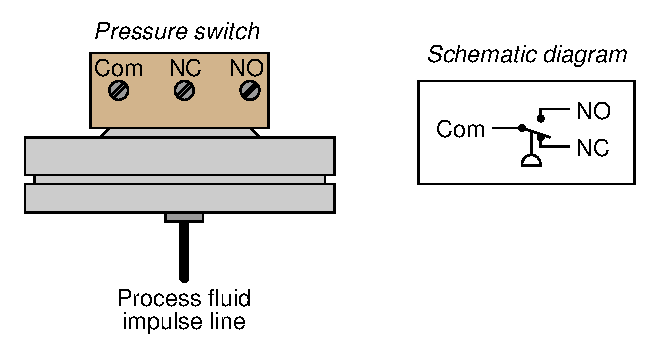
\includegraphics[width=15.5cm]{i00222x01.eps}$$

Forklar hva som menes med merkingen ``normalt lukket'' (NC) og ``normalt åpen'' (NO) ved to av de elektriske skruterminalene.  Angi bryterens status når prosesstrykket overstiger bryterens innstilte verdi.

\underbar{file i00222}
%(END_QUESTION)





%(BEGIN_ANSWER)

Som for alle prosessbrytere viser ``normal'' status til bryterens elektriske status ved {\it minimal påvirkning}.  I dette tilfellet, når prosesstrykket er under innstilt verdi, vil bryteren være i sin ``normal''-status (slik den er tegnet i skjemaet), med elektrisk kontinuitet mellom Com og NC, og ingen elektrisk kontinuitet mellom Com og NO.

\vskip 10pt

Det er svært viktig å skille mellom ``normal'' status for en prosessbryter og dens ``typiske'' status når den er installert i en fungerende prosess.  Hvis denne bryterens settpunkt for eksempel var 50 PSI, kunne vi bruke den som lavtrykksalarmbryter (PAL), med oppgave å aktivere alarm dersom prosesstrykket faller {\it under} 50 PSI.  Da ville alarmkretsen bruke Com- og NC-kontaktene, mens normalt prosesstrykk (over 50 PSI) holder den normalt lukkede kontakten i {\it åpen} tilstand, slik at kontakten faller tilbake til sin ``normale'' (lukkede) tilstand hvis prosesstrykket synker under 50 PSI.  Her vil NC-kontakten {\it vanligvis} stå åpen, selv om den er en ``normalt lukket'' kontakt, ganske enkelt på grunn av hvordan vi bruker den i prosessen.

Noen studenter kan reagere på denne konvensjonen: ``Hvorfor ikke kalle kontakten enten `normalt åpen' eller `normalt lukket' ut fra hvilken tilstand kontakten {\it vanligvis} står i under drift?''  Svaret er enkelt: bryterprodusenten vet ikke hvordan du skal bruke den.  Hvordan skulle produsenten vite om kontakten skal merkes NO eller NC hvis de ikke kjenner ``normal'' driftsbetingelse i prosessen din og formålet du vil bruke bryteren til?  Standardkonvensjonen med å definere ``normal'' kontaktstatus som tilstanden ved minimal påvirkning (lavt trykk for en trykkbryter, lav temperatur for en temperaturbryter osv.) kan virke forvirrende, men er faktisk mindre forvirrende enn alternativet mange studenter først ser for seg.

%(END_ANSWER)





%(BEGIN_NOTES)


%INDEX% Switch, pressure: ``normal'' status of contacts

%(END_NOTES)
